\section{Observation of Approximation Errors}
To study the character of approximation errors we first made a few experimental
observations on generated data.

\subsection{Data Generation}
\label{sec:data-generation}
Since we will later use the approximated histogram to estimate a genome size, 
we will mainly study Kmerlight's performance on the data that are to some
degree biologically plausible. We will base our data generation on a sequencing
process as it was described in section \ref{sec:sequencing}.

As the Kmerlight's input data consist of genome reads, we first generate a genome $g_1g_2g_3 \dots g_L$:
a random sequence of length $L$ consisting of characters $A, C, G, T$ each with probabilty $1/4$ at every position.

Aftewards we generate reads each of length $l=100$. Instead of creating an explicit number of reads, we choose
a parameter $c$ (coverage) and generate $c \cdot L / l$ independent reads.

To generate a single read we uniformly select a random starting position $s$ in genome from a range $1, \dots, L - l + 1$
and then the read consists of characters $g_s g_{s+1} \dots g_{s+l-1}$. Finally, to simulate sequencing errors,
we change each read character with probabilty $e/3$ ($e$ denotes error rate) into a one of the three other characters.

With parameters $L, c, e$ we are able to mimic the real squencing data and they provide us with suffucient freedom.

% TODO: link sources from covest github

\subsection{Error characteristics}

In this section we compare exact $k$-mer abundance histogram produced by Jellyfish software
to approximated histograms computed by Kmerlight (with parameters $t=7, r=2^{15}, u=2^{13}$ using 60MB of RAM).
We ran Kmerlight in 50 trials on the same input data and we investigate means and standard deviations of 
the estimates $\hat f_i$. We demostrate three error characteristics on a genome generated with parameters $L=10^6, c=50, e=0.02$.

\paragraph{Overestimation}
In figure \ref{img:exact-vs-approximated-histogram} it is clearly visible that Kmerlight systematically overestimates values of $f_i$.
Mean errors for abundances around 25 reach absolute values of 4000, which is 5\% relative error. Since these values $f_i$ are considerably
smaller than the number of all $k$-mers $F_0$, it is expected for the estimates $\hat f_i$ to have higher variance, but the bias of the
estimate ($E(\hat f_i) \neq f_i$) is unexpected and unexplained yet.  

In the following sections we clarify the source of this bias (\ref{sec:source-of-bias}) and we present means to make the estimator $\hat f_i$ unbiased (\ref{sec:unbiased-estimate}).

\begin{figure}
\centerline{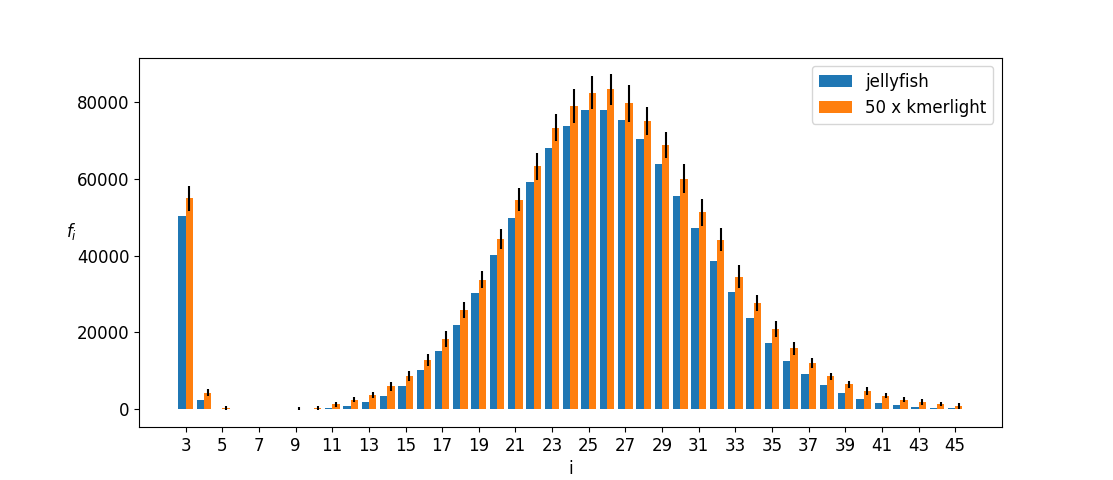
\includegraphics[width=1\textwidth, trim={1.5cm, 0cm, 2.5cm, 1.3cm}, clip]{{images/histogram_errors_L1000000_c50_e0.02_k21_normal}.png}}
\caption[Comparison of exact and approximated histograms]{Values of exact $f_i$ produced by Jellyfish software (blue)
and approximated values $\hat f_i$ produced by Kmerlight averaged from 50 trials (orange). The errorbars experss the
standard deviation of each estimate. Note that columns for $i=1,2$ were trimmed having values $10^7, 10^6$ respectively.}
\label{img:exact-vs-approximated-histogram}
\end{figure}

\paragraph{Higher variance and mean error with lower $f_i$}
Another characteristic of the errors is a trend of increasing variance and mean error of the estimates for lower values $f_i$.
In figure \ref{img:relative-errors} we visualize mean and standard deviation of relative errors $(\hat f_i - f_i) / f_i$ of $f_i$ estimates.
Kmerlight guarantees bounded errors only for most frequent $k$-mers, those with high $f_i/F_0$ ratio, but a theoretical qunatitative analysis of 
the error distribution was not presented in the previous work \cite{Sivadasan2016, Melsted2014}. 

We provide the quantitative estimate of the variance in section \ref{sec:estimation-variance} 
and then we use this knowledge to set Kmerlight's parameters to guarantee a specific error in \ref{sec:parameters-choice}.

\begin{figure}
\centerline{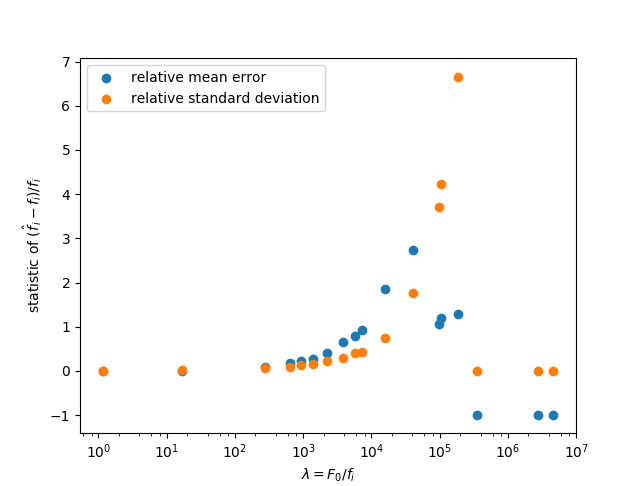
\includegraphics[width=0.8\textwidth, trim={0cm, 0cm, 0cm, 0cm}, clip]{{images/relative_errors_mean_std_L1000000_c50_e0.02_k21_normal}.png}}
\caption[Relative approximation errors]{Mean and standard deviation of relative errors $(\hat f_i - f_i) / f_i$ for columns sorted by decreasing $f_i$.
The drop in both statistics at values $\lambda = 10^5$ is caused by Kmerlight's insensitivity to infrequent $k$-mers.}
\label{img:relative-errors}
\end{figure}

\paragraph{Insensivity to lowest $f_i$}
Since the hash tables of Kmerlight's sketch are smaller than the number of all $k$-mers, many $k$-mers collide.
When the $k$-mer frequency $f_i$ reaches a specific boundary (in figure \ref{img:exact-vs-approximated-histogram-log} it seems to be $5 \times 10^3$), 
the probability that at least one $k$-mer with abundance $i$ becomes stored in a collision-free counter at any level approaches to 0.

As a result, the estimates $\hat f_i$ for the lowest $f_i$ may be based on none or very few counters with value $i$. Two scenarios may occur.
Either no $k$-mer survives the collisions ($t_i = 0$) and then is $\hat f_i = 0$, or very few $k$-mers survive the collisions. As the estimator
multiplies the number collision-free counters by factor $2^{w^*}$ ($\hat f_i \propto t_i \cdot 2^{w^*}$), the estimate may overestimate $f_i$ 
drastically if a higher level $w^*$ was selected.

This effect is expected, but we point it out as it may limit the usage of the approximated histogram to some applications.

\begin{figure}
\centerline{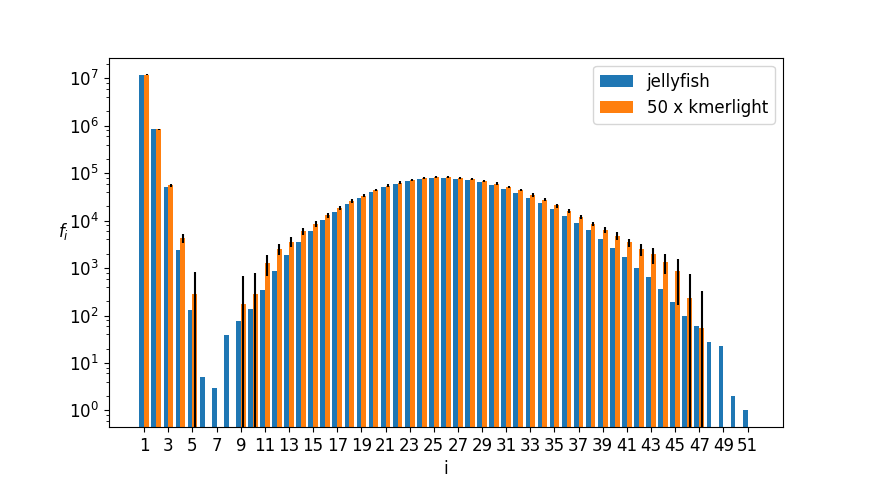
\includegraphics[width=1\textwidth, trim={2cm, 0cm, 2.5cm, 1.3cm}, clip]{{images/histogram_errors_L1000000_c50_e0.02_k21_normal_log}.png}}
\caption[Comparison of exact and approximated histograms in log scale]{Exact (blue) and average approximated (orange) histograms, identical
to those in figure \ref{img:exact-vs-approximated-histogram}, but displayed in a logarithmic scale with values $i=1, 2$ included. 
Note the lack of the orange columns where the blue columns reach lower values -- due to hashing collisions, Kmerlight can not estimate $f_i$ lower
than $5 \times 10^3$.}
\label{img:exact-vs-approximated-histogram-log}
\end{figure}
